\subsection{\acf{SAL}}
\label{subsec:AutonomousSensitiveArtificialListeners}

Schröder et al., developed a virtual agent integrated in SEMAINE~\cite{Schroder2010} called \acf{SAL} that has the required capabilities to sustain conversational dialogues and be a good listener~\cite{Schroder2012}.

\begin{figure}[H]
	\centering
	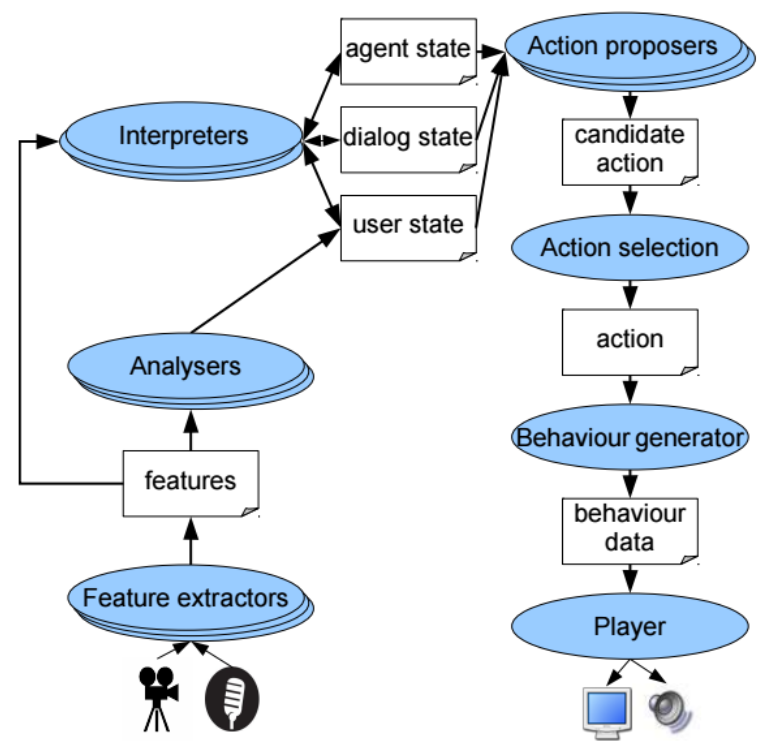
\includegraphics[width=0.45\textwidth]{images/SensitiveAgent.png}
	\caption{\acf{SAL} conceptual architecture. From~\cite{Schroder2012}.}
	\label{fig:sensitiveAgent}
\end{figure}


\subsubsection*{System Description}
Following the representation of the \ac{SAL} system in Figure~\ref{fig:sensitiveAgent}, the most relevant components are: \textit{Feature extractors}, \textit{Analysers}, \textit{Interpreters}, \textit{Action proposers}, and \textit{Action selection}. The \textit{Feature extractors} component extracts several features such as head gestures, facial features, emotions and, most of all, acoustic features. These features are later analysed by the \textit{Analysers} and \textit{Interpreters} components. The former component analyses non-verbal behaviours and speaker's emotions to produce an estimate of the information's reliability. The later component, given the information available, returns the best state representation for the user, dialogue and agent. Succeeding this, several \textit{Action proposers} propose an action, in parallel, given previous information. Following, the \textit{Action selection} component selects the action with the highest estimated quality, and lastly, the \textit{Behaviour generator} generates the desired action (utterances and facial animations).

Additionally, the agent is capable of identifying whether it should be in listener or in speaker mode. This is relevant as the \textit{Action selection} component gives more priority over speaker's actions. An example speaker action would be  saying ``Well?'' or ``Go on, tell me your news!'' after a long pause. In addition, in listener mode, the \textit{Action selection} component chooses the most suitable backchannel to be produced according to the emotions and interest level estimated from the user.

\subsubsection*{Evaluation}

The objective was to evaluate if emotion-related abilities influence the quality of human interactions. Firstly the users, with minimal \ac{HRI} experience, received an introductory briefing on the available personalities they can interact with (4 in total). Then, they interacted twice (random order) with each available personality: one with the expressive agent and the other with the affective features disabled. Afterwards, the user interacts with the \ac{SAL} agent's presented on a computer screen (only the face is rendered), using the available cameras and microphones.

\subsubsection*{Discussion}

There is evidence that expressive abilities may substantially impact the interactions between humans and agents by denoting that flow and perceived engagement was much higher in the emotional \ac{SAL} than in the control environment. Compared with previous systems, it presents the most complete model for managing backchannels and turn-taking strategies, however, as stated previously in Chapter~\ref{chap:rapport}, attentiveness and coordination are not enough to build rapport, it is also necessary to stimulate positivity which this system does not cover. To conclude, the most relevant aspects of the systems are:

\begin{itemize}
	\item Generation of good listener behaviour regardless of the content of the dialogue;
	\item Usage of parallel and independent action proposers that may either rule or \ac{ML} approaches;
	\item Usage of dedicated dialogue management models.
\end{itemize}